\chapter{От интегралов по траекториям к пропагаторам и вершинам}

Прежде чем перейти к перечню частиц и их взаимодействий, стоит прояснить основную конструкцию. Лагранжиан не только кодирует классические уравнения поля. Через интеграл по траекториям он также задаёт амплитуды того, как частицы распространяются, расщепляются, сливаются и рассеиваются. Это самый прямой путь от квантовой теории поля к диаграммам Фейнмана.

\section{Принцип наименьшего действия для частиц и полей}

Интеграл по траекториям Фейнмана — квантовый аналог принципа наименьшего действия. Начнём с обычной ньютоновской частицы, лагранжиан которой зависит от её координат и скоростей,
\begin{equation}
\mathcal{L}=\mathcal{L}(x,\dot{x}),
\end{equation}
а действие, сопоставляемое траектории, имеет вид
\begin{equation}
S[x]=\int \mathcal{L}(x,\dot{x})\,dt.
\end{equation}
Каждая пробная траектория от одной точки пространства-времени до другой имеет действие, независимо от того, удовлетворяет она уравнениям Ньютона или нет. Классическая траектория выделяется стационарностью действия. В традиционном языке ``наименьшего действия'' говорят, что она минимизирует действие, хотя более общее утверждение состоит именно в стационарности. Условие стационарности даёт классические дифференциальные уравнения движения.

\begin{figure}[htbp]
\centering
\includegraphics[width=0.72\textwidth]{lecture_10_figure_02.png}
\caption{Интеграл действия для траектории частицы.}
\lectureframe{00:02:14}
\end{figure}

Та же структура применима и к классическому полю. Будем обозначать все поля общим символом \(\phi\). Локальная плотность лагранжиана поля может зависеть от самих полей и от их пространственных и временных производных:
\begin{equation}
\mathcal{L}
=\mathcal{L}\!\left(\phi,\frac{\partial\phi}{\partial x^\mu}\right)
=\mathcal{L}(\phi,\partial_\mu\phi).
\end{equation}
Теория относительности требует, чтобы \(\mathcal{L}\) преобразовывался как скаляр Лоренца. При этом условии возможные члены лагранжиана задаются скалярными комбинациями полей и их производных.

\begin{figure}[htbp]
\centering
\includegraphics[width=0.62\textwidth]{lecture_10_figure_03.png}
\caption{Зависимость лагранжиана поля от поля и его пространственно-временных производных.}
\lectureframe{00:04:09}
\end{figure}

Для поля действие интегрируется по области пространства-времени:
\begin{equation}
S[\phi]=\int_{\Omega} d^4x\,\mathcal{L}(\phi,\partial_\mu\phi),
\qquad
d^4x=dt\,dx\,dy\,dz.
\end{equation}
Действие частицы — это интеграл по времени вдоль пути. Действие поля — это проинтегрированная по области пространства-времени плотность лагранжиана.

Аналогом фиксации концов траектории частицы служит задание полной конфигурации поля на начальном временном срезе и на конечном временном срезе. Если начальное поле равно \(\phi_{\mathrm{i}}(\mathbf{x})\), а конечное — \(\phi_{\mathrm{f}}(\mathbf{x})\), то интерполирующее поле заполняет весь слой пространства-времени между ними. Когда граничные данные допускают классическое интерполирующее решение, это решение является стационарной точкой действия при фиксированных граничных конфигурациях.
\editorialnote{Произвольные полные конфигурации поля на двух временных срезах не обязаны допускать классическое решение. Поэтому утверждение о стационарности действия ограничено теми граничными данными, для которых существует интерполирующее решение.}

Эта геометрия — полевотеоретический аналог траектории частицы.\footnote{Слой пространства-времени реконструирован по рисунку на доске примерно в 00:04:29.}
\begin{figure}[htbp]
\centering
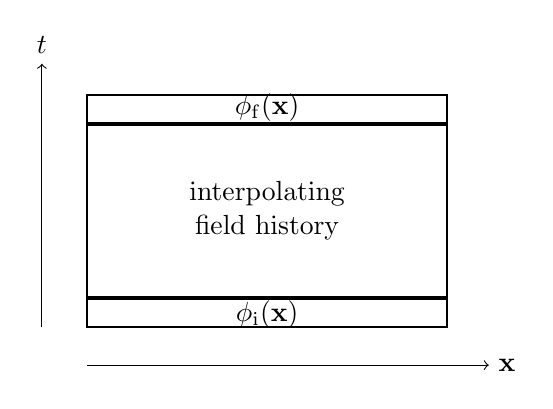
\begin{tikzpicture}[scale=0.88]
\draw[->] (-0.65,0) -- (-0.65,3.8) node[above] {$t$};
\draw[->] (0,-0.55) -- (5.8,-0.55) node[right] {$\mathbf{x}$};
\draw[thick] (0,0) rectangle (5.2,3.35);
\draw[very thick] (0,0.42) -- (5.2,0.42);
\draw[very thick] (0,2.93) -- (5.2,2.93);
\node at (2.6,0.18) {$\phi_{\mathrm{i}}(\mathbf{x})$};
\node at (2.6,3.17) {$\phi_{\mathrm{f}}(\mathbf{x})$};
\node[align=center] at (2.6,1.68) {interpolating\\field history};
\end{tikzpicture}
\caption{Начальная и конечная конфигурации поля, ограничивающие область пространства-времени.}
\end{figure}

\begin{classroomqa}
\lecturetimestamp{00:07:34}
\audiencequestion{Может ли поле вернуться к тому же значению?}
\lecturerresponse{Да. Ничто не мешает полю вернуться к более раннему значению, точно так же как ничто не мешает координате частицы вернуться к более раннему положению.}
\end{classroomqa}

\begin{classroomqa}
\lecturetimestamp{00:07:46}
\audiencequestion{Почему говорить о событиях пространства-времени или о траектории, если граничные данные — это значения поля?}
\lecturerresponse{Траектория частицы заменяется историей поля. Каждая конечная точка в пространстве полевых конфигураций — это всё поле на выбранном временном срезе, а история задаёт поле в каждой точке области пространства-времени между двумя срезами.}
\end{classroomqa}

Требование стационарности действия для интерполирующего поля приводит к уравнениям в частных производных. В зависимости от полей и лагранжиана среди них бывают, например, уравнения Максвелла и, для гравитационного действия, уравнения Эйнштейна. Подробный вариационный вывод здесь не нужен; важна следующая цепочка:
\begin{equation}
\mathcal{L}
\longrightarrow
S[\phi]
\longrightarrow
\text{classical field equations}.
\end{equation}

\section{Сумма Фейнмана по траекториям частицы}

Квантовая механика заменяет вопрос о том, какая траектория реализуется, вопросом об амплитудах. Представьте, что частицу вводят в \((x,t)\), на некоторое время закрывают глаза, а затем включают детектор в \((x',t')\). Амплитуда
\begin{equation}
\mathcal{A}(x,t;x',t')
\end{equation}
— комплексное число. Квадрат её модуля есть вероятность:
\begin{equation}
\begin{aligned}
P(x,t;x',t')
&=\left|\mathcal{A}(x,t;x',t')\right|^2\\
&=\mathcal{A}(x,t;x',t')
\mathcal{A}(x,t;x',t')^*.
\end{aligned}
\end{equation}

Правило Фейнмана сопоставляет каждой пробной траектории действие и ставит ей в соответствие фазу
\begin{equation}
\exp\!\left(-\frac{i}{\hbar}S[x]\right)
=
\exp\!\left[-\frac{i}{\hbar}\int \mathcal{L}(x,\dot{x})\,dt\right].
\end{equation}

\begin{figure}[htbp]
\centering
\includegraphics[width=0.70\textwidth]{lecture_10_figure_04.png}
\caption{Комплексная фаза, соответствующая траектории частицы.}
\lectureframe{00:11:52}
\end{figure}

Множитель \(\hbar\) необходим, чтобы показатель экспоненты был безразмерным.\footnote{При 00:11:52 запись на доске естественно читается как \(e^{-i\int\mathcal{L}\,dt}\); множитель \(\hbar\) добавляется устно при 00:12:02.} Амплитуда перехода равна сумме этих фаз по всем возможным путям, соединяющим конечные точки:
\begin{equation}
\mathcal{A}(x,t;x',t')
=
\sum_{\substack{\text{paths }x(\tau)\\(x,t)\rightarrow(x',t')}}
\exp\!\left(-\frac{i}{\hbar}S[x]\right).
\end{equation}
Здесь ``возможный путь'' не означает решение уравнений Ньютона. Это означает любой путь, входящий в сумму. В нерелятивистской квантовой механике пути идут вперёд по времени, а не возвращаются назад. Постоянная Планка имеет размерность действия, поэтому \(S/\hbar\) безразмерно.

Экспонента естественна, потому что амплитуды последовательных малых шагов перемножаются. Если путь разбить на последовательные участки, действие складывается,
\begin{equation}
S=S_1+S_2+\cdots,
\end{equation}
тогда как фазы перемножаются:
\begin{equation}
e^{-iS/\hbar}
=e^{-iS_1/\hbar}e^{-iS_2/\hbar}\cdots.
\end{equation}
Множитель \(i\) — не просто средство учёта; он является частью квантовомеханического правила.

\begin{classroomqa}
\lecturetimestamp{00:13:27}
\audiencequestion{Связана ли экспонента с перемножением амплитуд для последовательных малых шагов?}
\lecturerresponse{Да. Амплитуды последовательных шагов перемножаются, тогда как соответствующие части действия складываются.}
\end{classroomqa}

\begin{classroomqa}
\lecturetimestamp{00:13:49}
\audiencequestion{Является ли сама сумма по путям вероятностью?}
\lecturerresponse{Нет. Сумма по путям — это, вообще говоря, комплексная амплитуда вероятности. Умножение её на комплексно-сопряжённую величину даёт вероятность.}
\end{classroomqa}

\section{Сумма по историям поля}

Та же формулировка переносится и на квантовую теорию поля, хотя построение здесь будет намеренно нестрогим. Начнём с начальной конфигурации поля \(\phi(\mathbf{x})\) и отдельно заданной конечной конфигурации \(\phi'(\mathbf{x})\). Это полные функции пространства, а не значения в двух изолированных точках.

Можно вообразить идеализированный прибор, который задаёт поле в каждой пространственной точке, позволяет системе эволюционировать, а позже измеряет поле в каждой точке. Такой прибор нереалистичен, но он чётко формулирует концептуальный вопрос: какова амплитуда перехода от начальной полной конфигурации поля к конечной?

Вклад даёт каждая мыслимая интерполирующая история поля. Для каждой истории вычислите
\begin{equation}
S[\phi]=\int d^4x\,\mathcal{L}(\phi,\partial_\mu\phi)
\end{equation}
и сопоставьте соответствующую фазу. Схематически,
\begin{equation}
\mathcal{A}\!\left[\phi(\mathbf{x})\rightarrow\phi'(\mathbf{x})\right]
=
\sum_{\substack{\text{field histories}\\
\phi_{\mathrm{i}}=\phi,\;\phi_{\mathrm{f}}=\phi'}}
\exp\!\left(-\frac{i}{\hbar}S[\phi]\right).
\end{equation}
История не обязана удовлетворять классическим уравнениям поля. Это просто одно полное задание значений поля во всей промежуточной области пространства-времени.

\begin{classroomqa}
\lecturetimestamp{00:17:39}
\audiencequestion{Историй бесконечно много, и модуль каждой фазы равен 1. Как их сумма может сходиться? Минимизируются ли истории?}
\lecturerresponse{Истории суммируются, а не минимизируются. Члены суммы — это фазы, распределённые по единичной окружности, поэтому они могут взаимно сокращаться. Это отличается от сложения бесконечного числа положительных членов, отделённых снизу от нуля. Осциллирующие интегралы могут сходиться; привычный пример — фурье-представление дельта-функции. Если бы фазы были равномерно распределены по окружности, их векторная сумма обращалась бы в нуль. Большинство историй сильно гасят друг друга. Истории вблизи стационарной по действию истории гасят друг друга слабее всего, потому что там фаза меняется медленнее всего, и именно так возникает классический предел.}
\end{classroomqa}

\editorialnote{Интеграл по траекториям в реальном времени обычно требует предписания сходимости. Обсуждение единичной окружности даёт используемый здесь аргумент об осцилляционном сокращении, а не общее доказательство сходимости.}

Это взаимное сокращение можно наглядно представить как векторную сумму на комплексной плоскости.\footnote{Построение с единичной окружностью реконструировано по обсуждению у доски в 00:18:32--00:20:21.}
\begin{figure}[htbp]
\centering
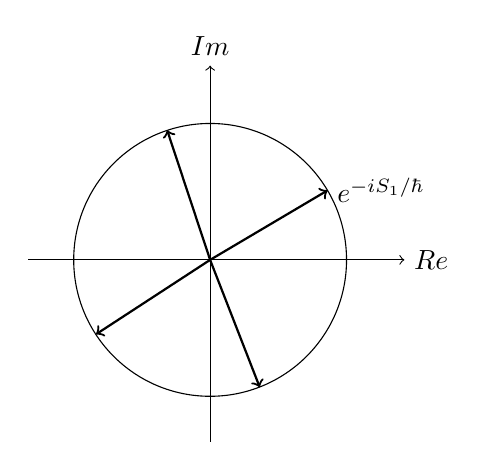
\begin{tikzpicture}[scale=1.05]
\draw[->] (-2.2,0) -- (2.35,0) node[right] {$\operatorname{Re}$};
\draw[->] (0,-2.2) -- (0,2.35) node[above] {$\operatorname{Im}$};
\draw (0,0) circle (1.65);
\draw[thick,->] (0,0) -- (1.42,0.84);
\draw[thick,->] (0,0) -- (-1.38,-0.90);
\draw[thick,->] (0,0) -- (-0.52,1.57);
\draw[thick,->] (0,0) -- (0.60,-1.54);
\node[right] at (1.42,0.84) {$e^{-iS_1/\hbar}$};
\end{tikzpicture}
\caption{Фазы единичного модуля могут взаимно сокращаться, если их направления различаются.}
\end{figure}

В самом деле,
\begin{equation}
e^{-iS/\hbar}
=
\cos\!\left(\frac{S}{\hbar}\right)
-i\sin\!\left(\frac{S}{\hbar}\right).
\end{equation}
Каждый вклад представляет собой единичный вектор. Вклады, направленные по-разному, не только складываются, но и вычитаются. Вблизи стационарной точки \(S\) соседние истории имеют почти одинаковую фазу, поэтому их вклады эффективнее усиливают друг друга. Вдали от стационарного действия фаза быстро меняется, и доминирует деструктивная интерференция.

Эта структура функционального интеграла лежит в основе практически всей современной квантовой теории поля. Следующий практический шаг будет сформулирован, а не выведен. Это чрезмерно упрощённый путь к вычислению, но он позволяет увидеть, как один и тот же объект может использоваться в двух языках описания.

Вычислить процесс — значит вычислить вероятность перехода из начального состояния в конечное. В одном описании задаются начальная и конечная конфигурации поля. В другом задаются входящие и выходящие частицы, кванты одного или нескольких полей. Эти вопросы выглядят по-разному, но оба вычисляются из одного и того же функционального интеграла теории поля.

\section{Дискретная форма пространства-времени}

Чтобы придать сумме по историям поля конкретный смысл, разделим пространство-время на малые ячейки и припишем каждой ячейке значение поля. Предел континуума достигается уменьшением размера ячеек, но пока они остаются конечными. Это превращает формальную сумму по функциям в сумму по всем присвоениям чисел ячейкам решётки.

Более ранняя эвристическая схема использует произведение множителей вида \(1+\mathcal{L}_i\), по одному для каждой ячейки, а затем выделяет члены, описывающие распространение и столкновение частиц. Эта конструкция достаточно важна, чтобы повторить её, но множитель нужно исправить. Малой величиной является не сам лагранжиан. Ею является действие, содержащееся в ячейке.

Если ячейка имеет пространственно-временной объём
\begin{equation}
a^4=\Delta t\,\Delta x\,\Delta y\,\Delta z,
\end{equation}
то её действие равно
\begin{equation}
A_i=\mathcal{L}_i a^4.
\end{equation}
Поскольку ячейка мала, мало и \(A_i\). Временно опуская \(\hbar\), получаем, что исправленный элементарный множитель имеет вид
\begin{equation}
1-iA_i,
\end{equation}
а не \(1+\mathcal{L}_i\).

Для любого малого \(\epsilon\),
\begin{equation}
1+\epsilon\simeq e^\epsilon,
\end{equation}
поскольку
\begin{equation}
e^\epsilon
=1+\epsilon+\frac{\epsilon^2}{2!}
+\frac{\epsilon^3}{3!}+\cdots.
\end{equation}
Следовательно, в этих временно выбранных единицах \(1-iA_i\) при достаточно малой ячейке приближённо равно \(e^{-iA_i}\). Удобнее с самого начала использовать точный экспоненциальный множитель.

\begin{classroomqa}
\lecturetimestamp{00:27:57}
\audiencequestion{Нужен ли в экспоненте множитель \(\hbar\)?}
\lecturerresponse{Да. Безразмерный множитель для ячейки в первом порядке равен \(1-iA_i/\hbar\), а точная экспонента имеет вид \(\exp(-iA_i/\hbar)\). Позже можно выбрать единицы, в которых \(\hbar=1\).}
\end{classroomqa}

После восстановления \(\hbar\) исправленный промежуточный множитель и его экспоненциальная форма имеют вид
\begin{equation}
1-\frac{i}{\hbar}A_i
\simeq
\exp\!\left(-\frac{i}{\hbar}A_i\right).
\end{equation}

Для фиксированной истории интеграл по пространству-времени заменяется суммой действий по ячейкам:
\begin{equation}
S[\phi]
=\int d^4x\,\mathcal{L}
\;\longrightarrow\;
\sum_i A_i.
\end{equation}
Фаза для этой истории становится равной
\begin{equation}
\exp\!\left(-\frac{i}{\hbar}\sum_i A_i\right).
\end{equation}
Экспонента от суммы есть произведение экспонент:
\begin{equation}
\exp\!\left(-\frac{i}{\hbar}\sum_i A_i\right)
=
\prod_i\exp\!\left(-\frac{i}{\hbar}A_i\right).
\end{equation}
Порядок действий важен. Сначала выбирают одну полную историю и перемножают её веса по ячейкам. Лишь затем суммируют по различным историям.

Решётка также делает явными граничные данные.\footnote{Шахматная доска и её фиксированные первая и последняя строки восстановлены по рисункам примерно на 00:23:54 и 00:30:49.}
\begin{figure}[htbp]
\centering
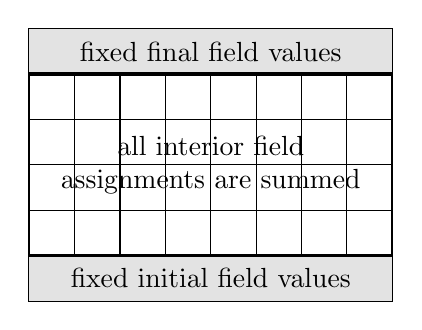
\begin{tikzpicture}[scale=0.72]
\draw[step=0.8,thin] (0,0) grid (6.4,4.8);
\draw[thick] (0,0) rectangle (6.4,4.8);
\fill[gray!22] (0,0) rectangle (6.4,0.8);
\fill[gray!22] (0,4.0) rectangle (6.4,4.8);
\draw[very thick] (0,0.8) -- (6.4,0.8);
\draw[very thick] (0,4.0) -- (6.4,4.0);
\node at (3.2,0.4) {fixed initial field values};
\node at (3.2,4.4) {fixed final field values};
\node[align=center] at (3.2,2.4) {all interior field\\assignments are summed};
\end{tikzpicture}
\caption{Дискретные истории поля с фиксированными начальной и конечной строками решётки.}
\end{figure}

Первая строка задаёт начальную конфигурацию поля, а последняя строка — конечную. Каждая внутренняя ячейка может принимать любое значение поля, входящее в дискретизацию. Поэтому амплитуда перехода схематически имеет вид
\begin{equation}
\mathcal{A}\!\left[\phi_{\mathrm{i}}\rightarrow\phi_{\mathrm{f}}\right]
=
\sum_{\{\phi\}_{\mathrm{interior}}}
\prod_i\exp\!\left(-\frac{i}{\hbar}A_i[\phi]\right),
\end{equation}
при фиксированных первой и последней строках. Эквивалентно, для каждого внутреннего присвоения вычисляют экспоненту полного действия, а затем складывают этот вклад со вкладами всех остальных присвоений.

\section{От конфигураций поля к конфигурациям частиц}

Одну и ту же амплитуду перехода можно описывать в терминах полей или в терминах частиц. Вместо того чтобы фиксировать поле на первом и последнем временных слоях, можно задать входящий набор квантов поля и выходящий набор таких квантов, а затем спросить об амплитуде, связывающей их. Вычисляемый объект остаётся тем же самым. Изменилось только граничное описание.

Квантовые поля содержат операторы рождения и уничтожения. Поэтому произведения полей действуют на состояния частиц, рождая, уничтожая или перемещая кванты. Именно такая операторная интерпретация превращает решёточный функциональный интеграл в набор правил для частиц.

\begin{classroomqa}
\lecturetimestamp{00:34:11}
\audiencequestion{Обязательно ли кванты поля можно отождествить с частицами?}
\lecturerresponse{Не всегда — в обычном смысле частиц, наблюдаемых по отдельности. Например, кварки являются квантами кварковых полей, но конфайнмент не позволяет изолированному кварку вырваться и быть обнаруженным сам по себе. Более общо, между полями, фигурирующими в теории, и видами частиц, которые выступают как обычные наблюдаемые состояния, не обязано существовать взаимно-однозначное соответствие. Некоторые теории поля не допускают такого простого соответствия. Если ``частица'' употребляется в широком смысле как неделимый квант, несущий энергию и другие квантовые числа, то это различие отчасти может стать вопросом терминологии.}
\end{classroomqa}

\editorialnote{Оговорка источника о слабой связи в 00:35:45--00:36:08 грамматически неоднозначна и здесь оставлена без разрешения. Надёжное утверждение состоит в том, что обозначения полей и виды частиц, обычно наблюдаемые как экспериментальные состояния, не обязаны находиться во взаимно-однозначном соответствии.}

Сама сумма по решётке по-прежнему берётся по значениям поля. Она не ограничивается конфигурациями, похожими на гладкие классические решения.

\begin{classroomqa}
\lecturetimestamp{00:36:44}
\audiencequestion{Должны ли истории поля быть непрерывными или хотя бы приближённо непрерывными?}
\lecturerresponse{Нет. На дискретной решётке соседние ячейки просто несут значения поля, и в сумму включается каждое присвоение. Никакого ограничения на истории, которые приблизительно непрерывны, нет. Квантовые поля сильно флуктуируют; типичные истории не являются гладкими классическими полями.}
\end{classroomqa}

Независимо задаваемыми переменными являются поля в узлах или ячейках решётки. Их производные получают из разностей между соседними значениями.

\begin{classroomqa}
\lecturetimestamp{00:37:56}
\audiencequestion{Задаются ли независимо значения полей и их производных?}
\lecturerresponse{Нет. Значения полей задаются в узлах. Затем производная восстанавливается по разности между соседними значениями поля. Возможны различные конечно-разностные схемы, но производные не являются дополнительными независимыми переменными.}
\end{classroomqa}

Таким образом, при шаге решётки \(a\) можно схематически написать
\begin{equation}
\partial_\mu\phi(x)
\longrightarrow
\frac{\phi(x+a\hat\mu)-\phi(x)}{a}.
\end{equation}
Сама ось значений поля тоже может быть разбита на малые интервалы, так что в каждом узле остаётся счётное множество возможных значений.

\begin{classroomqa}
\lecturetimestamp{00:38:53}
\audiencequestion{Что меняется, если полей больше одного?}
\lecturerresponse{В каждом узле задаётся значение каждого поля, и сумма берётся по всем таким присвоениям.}
\end{classroomqa}

Поле с комплексными значениями не следует путать с аналитической функцией комплексной переменной. Аналитичность — исключительно сильное условие гладкости. Истории в функциональном интеграле по полям не обязаны ему удовлетворять и, вообще говоря, даже не являются приблизительно гладкими.

\begin{classroomqa}
\lecturetimestamp{00:39:07}
\audiencequestion{Если поля принимают комплексные значения, должны ли их значения удовлетворять условиям гладкости, которым подчиняются аналитические функции?}
\lecturerresponse{Нет. Комплекснозначность не означает аналитичности. Теория аналитических функций касается чрезвычайно гладкого и жёстко ограниченного класса функций. Суммируемые здесь истории поля не обязаны быть аналитическими функциями координат; типичные истории крайне нерегулярны и в пределе континуума могут рассматриваться как сильно разрывные.}
\end{classroomqa}

Получающееся вычисление выглядит устрашающе сложным. Даже после дискретизации пространства-времени и значений поля число присвоений, из которых нужно делать выборку, может быть огромным.

\begin{classroomqa}
\lecturetimestamp{00:40:04}
\audiencequestion{Как компьютер узнаёт, сколько решёточных присвоений нужно включить в выборку и когда расчёт сошёлся?}
\lecturerresponse{Этот вопрос относится к решёточной калибровочной теории или, более общо, к решёточной квантовой теории поля. К настоящему времени это уже эффективная вычислительная дисциплина. Я участвовал в самом начале в установлении правил решёточной калибровочной теории, а не в более поздних компьютерных технологиях. На выработку правил ушло около трёх недель; на развитие технологии вычисления таких вещей — что-то вроде 30 лет. Большая часть практической мудрости пришла из статистической механики, где статистические суммы тоже получают суммированием по конфигурациям решётки---например, по тому, занят ли узел в кристалле. Определение того, достаточно ли конфигураций попало в выборку, — технический вопрос. Эксперты знают---или думают, что знают---когда расчёт находится под контролем, и получающиеся результаты согласуются с экспериментом.}
\end{classroomqa}

Концептуальные правила решёточной калибровочной теории появились быстро; технология, необходимая для вычислений с их помощью, потребовала гораздо больше времени. Шахматная доска — не просто аналогия. Это также исходный пункт практического вычислительного метода.

\section{Квадратичные члены и распространение частиц}

Теперь вернёмся к операторной интерпретации полей. Для двух соседних узлов \(x\) и \(x'\) произведение
\begin{equation}
\phi(x)\phi(x')
\end{equation}
может в подходящем одночастичном матричном элементе обеспечивать уничтожение частицы в одном узле и её создание в другом. Поэтому в этом секторе его можно изображать как переход по одному звену. Это лишь одна интерпретация операторного произведения, а не его единственный смысл.

Члены, отвечающие за такие связи, — это члены с производными. Строго говоря, они связаны не с одной ячейкой, а с соседней парой. Временная производная, например, принимает вид
\begin{equation}
\partial_t\phi(t,\mathbf{x})
\longrightarrow
\frac{\phi(t+a,\mathbf{x})-\phi(t,\mathbf{x})}{a},
\end{equation}
и пространственная производная обрабатывается таким же образом вдоль пространственного звена.

\begin{classroomqa}
\lecturetimestamp{00:44:39}
\audiencequestion{Содержат ли обсуждаемые лагранжианы вторые производные?}
\lecturerresponse{Рассматриваемые здесь стандартные теории записываются с первыми производными. Поэтому в их решёточных версиях используются первые разности между соседними узлами.}
\end{classroomqa}

Возведение первой разности в квадрат даёт и одноузловые члены, и перекрёстный член для соседних узлов:
\begin{align}
\frac{1}{2}\bigl[\phi(x)-\phi(x')\bigr]^2
&=
\frac{1}{2}\phi(x)^2
+\frac{1}{2}\phi(x')^2
-\phi(x)\phi(x').
\end{align}
Перекрёстный член может обеспечивать переход из одного узла в другой. Два квадрата — это одноузловые члены. Квадратичные члены с производными являются кинетическими членами, и именно их перекрёстные члены по соседним узлам мы сначала будем использовать для построения распространения.

Чтобы выделить комбинаторику, соберём произведения по соседним узлам в
\begin{equation}
K=\sum_{\langle x,x'\rangle}\phi(x)\phi(x').
\end{equation}
Соответствующий множитель в весе функционального интеграла схематически записывается как
\begin{equation}
e^{-iK}.
\end{equation}
\editorialnote{В этом схематическом решёточном множителе опущены степени шага решётки, \(\hbar\), знаки метрики, нормировочные константы и коэффициенты при звеньях.}
Его разложение имеет вид
\begin{equation}
e^{-iK}
=1-iK-\frac{1}{2!}K^2+\frac{i}{3!}K^3+\cdots,
\end{equation}
или, если явно выписать суммы по соседним узлам,
\begin{align}
e^{-iK}
={}&1
-i\sum_{\langle x,x'\rangle}\phi(x)\phi(x')
\nonumber\\
&-\frac{1}{2!}
\sum_{\langle x,x'\rangle}
\sum_{\langle y,y'\rangle}
\phi(x)\phi(x')\phi(y)\phi(y')
+\cdots .
\end{align}
Каждый множитель независимо выбирает соседнюю пару.

Диаграммы частиц подчиняются правилу отсутствия висячих концов. Открытый конец допустим только там, где граничное условие явно вводит частицу на начальном слое или удаляет её на конечном. Изолированное звено внутри области имеет несогласованные концы и не представляет полного вклада в заданный переход. Внутренние концы звеньев должны соединяться.

Рассмотрим сначала решётку высотой всего в два временных слоя. Если начальное состояние вводит частицу в \(x\), а конечное состояние удаляет её в соседней точке \(x'\), то член первого порядка может соединить эти две граничные вставки:
\begin{equation}
x\longrightarrow x',
\qquad
\mathcal{A}_{\text{one link}}\sim -i.
\end{equation}
Коэффициент \(-i\) — это лишь коэффициент в этом схематическом разложении; при этом по-прежнему подразумеваются опущенные решёточные и нормировочные множители.

\begin{classroomqa}
\lecturetimestamp{00:52:16}
\audiencequestion{Вносит ли член первого порядка с одним звеном вклад только тогда, когда соответствующие начальный и конечный узлы соседние?}
\lecturerresponse{Да. Этот член выбирает одну соседнюю пару, так что он может соединить эти граничные узлы только в том случае, если они соседние. Распространение на большее расстояние возникает из произведений более высокого порядка.}
\end{classroomqa}

Во втором порядке два множителя независимо суммируются по соседним парам:
\begin{equation}
K^2
=
\sum_{\langle x,x'\rangle}
\sum_{\langle y,y'\rangle}
\phi(x)\phi(x')\phi(y)\phi(y').
\end{equation}

\begin{classroomqa}
\lecturetimestamp{00:52:40}
\audiencequestion{Должна ли вторая соседняя пара примыкать к паре, выбранной первым множителем?}
\lecturerresponse{Нет. Каждый множитель независимо выбирает соседнюю пару. Две пары могут иметь общий узел, могут быть полностью раздельными или даже совпадать, то есть быть одной и той же парой. Сумма включает все возможности.}
\end{classroomqa}

Для распространения одной частицы через три временных слоя полезный выбор второго порядка имеет общий промежуточный узел:
\begin{equation}
\bigl[\phi(x_0)\phi(x_1)\bigr]
\bigl[\phi(x_1)\phi(x_2)\bigr],
\qquad
x_0\longrightarrow x_1\longrightarrow x_2.
\end{equation}
Конец первого звена соединён с началом второго. Открытыми остаются только начальная точка \(x_0\) и конечная точка \(x_2\), поэтому этот член вносит вклад в требуемый одночастичный переход. В схематической экспоненте его коэффициент равен
\begin{equation}
-\frac{1}{2!}.
\end{equation}

Вместо этого выбранные пары могут образовывать отдельные переходы.\footnote{Диаграммы звеньев восстановлены по фрагменту 00:49:18--00:55:12.}
\begin{figure}[htbp]
\centering
\resizebox{\linewidth}{!}{%
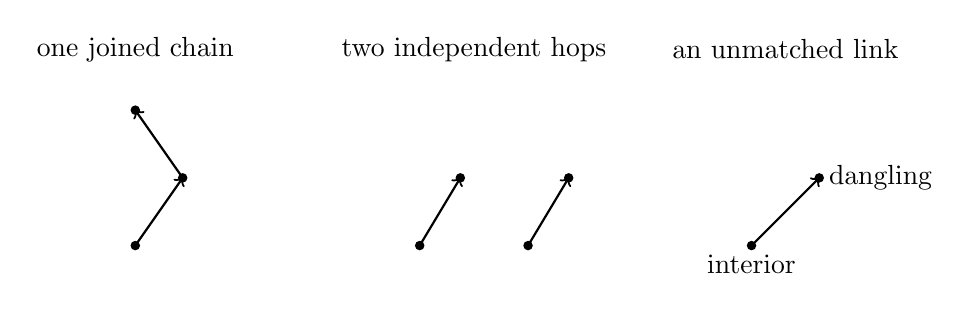
\begin{tikzpicture}[scale=0.86]
\node at (0,2.9) {one joined chain};
\fill (0,0) circle (2pt);
\fill (0.7,1.0) circle (2pt);
\fill (0,2.0) circle (2pt);
\draw[thick,->] (0,0) -- (0.7,1.0);
\draw[thick,->] (0.7,1.0) -- (0,2.0);

\begin{scope}[xshift=4.2cm]
\node at (0.8,2.9) {two independent hops};
\fill (0,0) circle (2pt);
\fill (0.6,1.0) circle (2pt);
\fill (1.6,0) circle (2pt);
\fill (2.2,1.0) circle (2pt);
\draw[thick,->] (0,0) -- (0.6,1.0);
\draw[thick,->] (1.6,0) -- (2.2,1.0);
\end{scope}

\begin{scope}[xshift=9.1cm]
\node at (0.5,2.9) {an unmatched link};
\fill (0,0) circle (2pt);
\fill (1.0,1.0) circle (2pt);
\draw[thick,->] (0,0) -- (1.0,1.0);
\node[below] at (0,0) {interior};
\node[right] at (1.0,1.0) {dangling};
\end{scope}
\end{tikzpicture}%
}
\caption{Соединённое, независимое и несогласованное выделение соседних звеньев.}
\end{figure}

Уже в этом порядке может существовать более одного маршрута. Для смещения на один временной и один пространственный шаг решётки два порядка
\begin{align}
x
&\longrightarrow x+\hat t
\longrightarrow x+\hat t+\hat s,\\
x
&\longrightarrow x+\hat s
\longrightarrow x+\hat s+\hat t
\end{align}
приводят к одной и той же конечной точке.

\begin{classroomqa}
\lecturetimestamp{00:55:53}
\audiencequestion{Есть ли другой двухшаговый путь к той же диагональной конечной точке?}
\lecturerresponse{Да. Можно сначала сделать временной шаг, а затем пространственный, или выполнить их в обратном порядке. Оба маршрута вносят вклад в одну и ту же амплитуду перехода.}
\end{classroomqa}

Нет причин останавливаться на двух звеньях. Член третьего порядка даёт цепочки из трёх соседних звеньев. Маршрут может продвигаться прямо, делать обход или сначала удаляться, а затем возвращаться, прежде чем достигнуть конечной точки. Ещё более высокие порядки включают более длинные обходы и повторные обратные ходы. Поэтому разложение до произвольного порядка даёт вклад для каждого маршрута, составленного из локальных звеньев. Амплитуда перехода из точки в точку есть сумма всех этих вкладов, с коэффициентами, содержащими соответствующие степени \(i\) и факториалы:
\begin{equation}
\begin{gathered}
\mathcal{A}(x_{\mathrm{in}}\to x_{\mathrm{out}})
=
\sum_{\text{joined lattice routes }r}c_r,
\\
c_r\ \hbox{read from the exponential expansion}.
\end{gathered}
\end{equation}
Коэффициенты, вообще говоря, комплексны, так что и получающаяся амплитуда комплексна.

Релятивистское распространение добавляет ещё одну возможность. Маршрут может идти и вверх, и вниз по времени, а также многократно проходить по одному и тому же звену.

\begin{classroomqa}
\lecturetimestamp{00:58:47}
\audiencequestion{Может ли путь снова и снова проходить через одни и те же две ячейки?}
\lecturerresponse{Да. Повторные прохождения включены, и в релятивистском разложении маршрут может также идти назад по времени.}
\end{classroomqa}

Отрезок с обратным ходом по времени допускает два эквивалентных графических прочтения. Его можно трактовать как линию частицы, идущую назад по времени. Или же можно рассматривать время только вперёд: создаётся пара частица--античастица, частица продолжает двигаться вперёд, а античастица позже встречается с исходной частицей и аннигилирует с ней. Одна и та же связная линия кодирует оба описания.\footnote{Оба прочтения следуют из диаграммы и объяснения в 00:59:00--00:59:51.}

\begin{figure}[htbp]
\centering
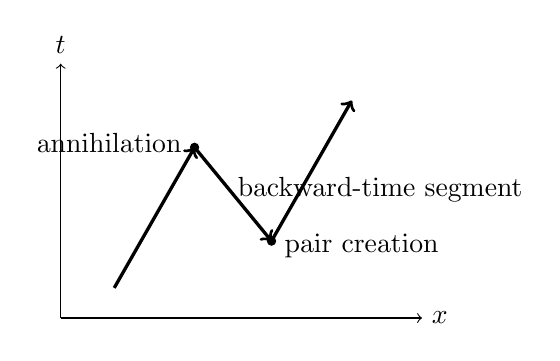
\begin{tikzpicture}[scale=0.85]
\draw[->] (0,0) -- (0,3.8) node[above] {$t$};
\draw[->] (0,0) -- (5.4,0) node[right] {$x$};
\draw[very thick,->] (0.8,0.45) -- (2.0,2.55);
\draw[very thick,->] (2.0,2.55) -- (3.15,1.15);
\draw[very thick,->] (3.15,1.15) -- (4.35,3.25);
\fill (2.0,2.55) circle (2pt);
\fill (3.15,1.15) circle (2pt);
\node[left] at (1.95,2.62) {annihilation};
\node[right] at (3.20,1.08) {pair creation};
\node[right] at (2.50,1.92) {backward-time segment};
\end{tikzpicture}
\caption{Отрезок с обратным ходом по времени, читаемый вперёд как рождение и аннигиляция пары.}
\end{figure}

Факториалы, появляющиеся на высоких порядках, управляют экспоненциальным степенным рядом, но это не то же самое, что контролировать полную сумму по конфигурациям поля.

\begin{classroomqa}
\lecturetimestamp{01:00:00}
\audiencequestion{Гарантируют ли множители \(1/n!\) сходимость?}
\lecturerresponse{Они гарантируют сходимость экспоненциального ряда при фиксированном аргументе. Сами по себе они не гарантируют сходимости отдельной суммы по всем конфигурациям поля. Это разные вопросы. На конечной решётке с конечным дискретизированным набором значений поля число конфигураций конечно, но пределы континуума и бесконечного объёма требуют дополнительного контроля.}
\end{classroomqa}

\section{Произведение на одном звене и несколько интерпретаций в терминах частиц}

Член второго порядка содержит не только одночастичное распространение. Когда две соседние пары имеют общий конец, он может перемещать одну частицу по цепочке из двух звеньев:
\begin{equation}
\bigl[\phi(x_0)\phi(x_1)\bigr]
\bigl[\phi(x_1)\phi(x_2)\bigr].
\end{equation}
Когда выбранные пары раздельны, тот же член второго порядка может перемещать две частицы, каждую на одно звено.\footnote{Сопоставление одночастичного распространения и двух независимых переходов по одному звену восстановлено по обсуждению у доски в 01:00:46--01:02:34.}
\begin{equation}
\bigl[\phi(x_0)\phi(x_1)\bigr]
\bigl[\phi(y_0)\phi(y_1)\bigr],
\qquad x_0\neq y_0.
\end{equation}
Первый множитель переносит одну частицу, а второй — другую. Таким образом, квадратичное решёточное разложение содержит амплитуды распространения во всех многочастичных секторах. Один и тот же алгебраический порядок может описывать один более длинный связный маршрут или несколько более коротких несвязанных маршрутов.

Это очень большой объём информации, но это ещё не настоящая вершина взаимодействия. При наличии только квадратичных членов распространения связные линии частиц не расщепляются в другое число линий. Процессы с изменением числа частиц требуют дополнительных взаимодействий, хотя локальные операторные произведения и могут допускать несколько прочтений в терминах рождения и уничтожения.

\begin{classroomqa}
\lecturetimestamp{01:03:30}
\audiencequestion{Могут ли электрон и позитрон аннигилировать, не оставив вообще никаких частиц?}
\lecturerresponse{Вклад с ненулевой входящей энергией и без конечного состояния, переносящего энергию, нарушает закон сохранения энергии. При суммировании по всем его возможным положениям в пространстве-времени амплитуды взаимно сокращаются. Электрон--позитронная аннигиляция может происходить, когда другое поле уносит энергию---например, при рождении электромагнитных квантов.}
\end{classroomqa}

\editorialnote{Сокращённое обсуждение сразу переходит от квадратичного перескока к электрон--позитронной аннигиляции. Существенное различие здесь состоит в том, что квадратичные члены задают свободное распространение, тогда как физическая аннигиляция требует взаимодействия с другим полем; амплитуда без выходных частиц обнуляется вследствие сохранения энергии.}

Таким образом, члены с производными определяют многое, но не всё. Дальнейшие члены лагранжиана определяются экспериментально наблюдаемыми свойствами и взаимодействиями полей.

\section{Массовый член}

Для скалярного поля обсуждаемая структура производных имеет схематическую лоренцевскую сигнатуру
\begin{equation}
\mathcal{L}_{\mathrm{kin}}
\sim
\frac{1}{2}\left[
(\partial_t\phi)^2
-(\partial_x\phi)^2
-(\partial_y\phi)^2
-(\partial_z\phi)^2
\right].
\end{equation}
Это выражение фиксирует существенную для обсуждения структуру «временная минус пространственная»; общие знаки и соглашения о нормировке оставлены неявными.

Лагранжиан может также содержать степени поля без производных. Квадратичный пример имеет вид
\begin{equation}
\text{mass term}\ \propto\ \frac{1}{2}m^2\phi^2,
\end{equation}
где \(m^2\) отождествляется с коэффициентом массы.\editorialnote{В этом фрагменте источник не фиксирует соглашение об общем знаке для полного скалярного лагранжиана.} В схематической интерпретации в терминах частиц этот член уничтожает частицу и вновь создаёт её в том же узле решётки. Он не смещает частицу. Он вставляет в путь множитель в том же узле:
\begin{equation}
\text{particle at }x
\longrightarrow
\boxed{m^2\phi(x)^2}
\longrightarrow
\text{particle still at }x.
\end{equation}
Каждый раз, когда действует такая вставка, путь приобретает ещё один множитель, пропорциональный \(m^2\).

Если оставить только члены с производными, то получающееся распространение в этой схематической развертке соответствует безмассовой теории. Для массивного поля путь может включать любое число массовых вставок в том же узле между членами перескока. Массовый член изменяет относительные веса путей так, что результирующий пропагатор несёт массу частицы.

\section{Кубические члены и истории расщепления--воссоединения}

Массовый член изменяет вес пути, не перемещая частицу. Более интересное поведение начинается с членов степени выше второй. Возьмём кубическое взаимодействие,
\begin{equation}
\mathcal{L}_{\mathrm{int}}=g_3\phi^3.
\end{equation}
В одной ячейке решётки эти три множителя поля допускают четыре интерпретации в терминах частиц:
\begin{equation}
1\longrightarrow 2,
\qquad
2\longrightarrow 1,
\qquad
0\longrightarrow 3,
\qquad
3\longrightarrow 0.
\end{equation}
Таким образом, кубический множитель может уничтожить одну частицу и создать две, уничтожить две и создать одну, создать три или уничтожить три.

Квадратичные множители соседних пар по-прежнему обеспечивают распространение. Их последовательность может перенести частицу в ячейку, кубический множитель в этой ячейке может поглотить её и испустить две частицы, а дальнейшие квадратичные множители могут унести эти две частицы дальше. Это даёт вклад в амплитуду процесса с одной входящей и двумя выходящими частицами.\footnote{Геометрия решётки восстановлена по диаграмме на 01:08:48--01:09:42.}

\begin{figure}[htbp]
\centering
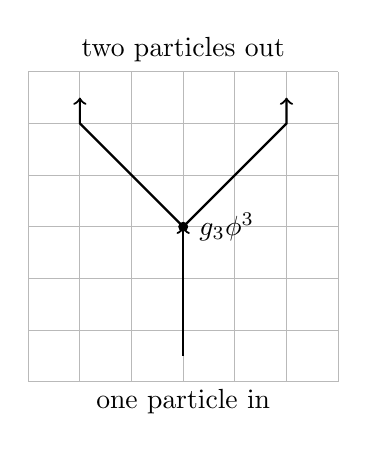
\begin{tikzpicture}[scale=0.82]
\draw[step=0.8,gray!55,thin] (0,0) grid (4.8,4.8);
\draw[thick,->] (2.4,0.4) -- (2.4,1.2) -- (2.4,2.0) -- (2.4,2.4);
\fill (2.4,2.4) circle (2.2pt);
\draw[thick,->] (2.4,2.4) -- (1.6,3.2) -- (0.8,4.0) -- (0.8,4.4);
\draw[thick,->] (2.4,2.4) -- (3.2,3.2) -- (4.0,4.0) -- (4.0,4.4);
\node[right] at (2.5,2.4) {$g_3\phi^3$};
\node at (2.4,-0.3) {one particle in};
\node at (2.4,5.15) {two particles out};
\end{tikzpicture}
\caption{Квадратичные множители обеспечивают распространение частицы к кубической вершине расщепления и от неё.}
\end{figure}

Даже амплитуда с одной частицей и в начальном, и в конечном состоянии уже не является просто суммой одиночных непрерывных путей. Один вклад даёт прямое распространение по цепочке квадратичных перескоков. Другой вклад содержит два кубических множителя: частица расщепляется на две, а эти две позже вновь соединяются. Поэтому промежуточное состояние может содержать больше частиц, чем внешнее состояние.\footnote{Обе альтернативы восстановлены по диаграмме на 01:09:44--01:11:36.}

\begin{figure}[htbp]
\centering
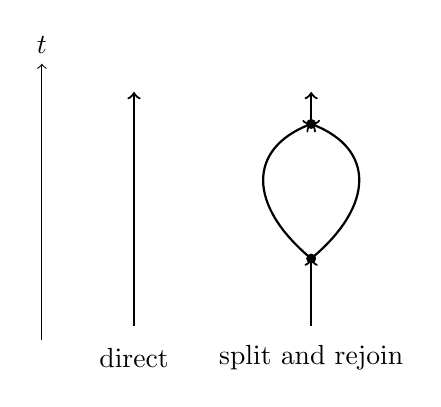
\begin{tikzpicture}[scale=0.9]
\draw[->] (-0.7,0) -- (-0.7,3.9) node[above] {$t$};
\draw[thick,->] (0.6,0.2) -- (0.6,3.5);
\node at (0.6,-0.25) {direct};
\draw[thick,->] (3.1,0.2) -- (3.1,1.15);
\fill (3.1,1.15) circle (2pt);
\draw[thick,->] (3.1,1.15) .. controls (2.2,1.9) and (2.2,2.7) .. (3.1,3.05);
\draw[thick,->] (3.1,1.15) .. controls (4.0,1.9) and (4.0,2.7) .. (3.1,3.05);
\fill (3.1,3.05) circle (2pt);
\draw[thick,->] (3.1,3.05) -- (3.1,3.5);
\node at (3.1,-0.25) {split and rejoin};
\end{tikzpicture}
\caption{Прямое распространение и вклад расщепления--воссоединения в одну и ту же одночастичную амплитуду.}
\end{figure}

В электродинамике соответствующий пример — электрон, который испускает фотон, а позже вновь поглощает его. Эта история с испусканием и повторным поглощением входит в амплитуду распространения электрона из одной точки в другую. В более высоких порядках встречаются несколько актов испускания и поглощения. Фотон может превратиться в электрон--позитронную пару, а электрон и позитрон в этой промежуточной паре могут и сами обменяться фотоном. Ничто не требует, чтобы промежуточный состав частиц был простым лишь потому, что начальный и конечный составы частиц просты.\footnote{Примеры в следующей реконструкции появляются на 01:11:22--01:12:34.}

\begin{figure}[htbp]
\centering
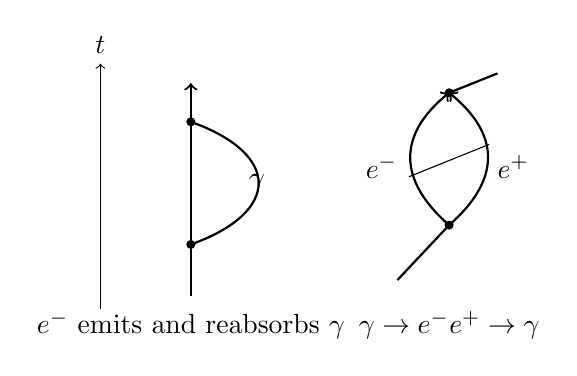
\begin{tikzpicture}[scale=0.82]
\draw[->] (-0.6,0) -- (-0.6,3.8) node[above] {$t$};
\draw[thick,->] (0.8,0.2) -- (0.8,3.5);
\fill (0.8,1.0) circle (2pt);
\fill (0.8,2.9) circle (2pt);
\draw[thick] (0.8,1.0) .. controls (2.2,1.5) and (2.2,2.4) .. (0.8,2.9);
\node[right] at (1.55,1.95) {$\gamma$};
\node at (0.8,-0.25) {$e^-$ emits and reabsorbs $\gamma$};
\draw[thick] (4.0,0.45) -- (4.8,1.3);
\fill (4.8,1.3) circle (2pt);
\draw[thick,->] (4.8,1.3) .. controls (4.0,2.0) and (4.0,2.7) .. (4.8,3.35);
\draw[thick,->] (4.8,1.3) .. controls (5.6,2.0) and (5.6,2.7) .. (4.8,3.35);
\fill (4.8,3.35) circle (2pt);
\draw[thick] (4.8,3.35) -- (5.55,3.65);
\draw[thin] (4.18,2.05) -- (5.42,2.55);
\node[left] at (4.15,2.2) {$e^-$};
\node[right] at (5.4,2.2) {$e^+$};
\node at (4.8,-0.25) {$\gamma\to e^-e^+\to\gamma$};
\end{tikzpicture}
\caption{Вклад от самоиспускания электрона и история фотона, содержащая электрон--позитронную пару.}
\end{figure}

Каждая такая история возникает из определённого произведения членов в разложении экспоненты. Её коэффициент несёт соответствующую степень \(i\), факториал из ряда экспоненты и константы связи, присоединённые к её вершинам. Этот коэффициент даёт вклад данной истории, но амплитуда для заданных начального и конечного состояний есть сумма всех историй с теми же внешними состояниями.

\begin{classroomqa}
\lecturetimestamp{01:13:18}
\audiencequestion{Может ли один и тот же общий процесс происходить через несколько разных историй, так что все они вносят вклад в его амплитуду?}
\lecturerresponse{Да. Амплитуда процесса получается из всех различных историй, соединяющих одно и то же начальное состояние с одним и тем же конечным состоянием.}
\end{classroomqa}

Итак, существуют два эквивалентных способа организовать квантовую теорию поля. В полевом описании задают начальную и конечную конфигурации поля и суммируют по всем промежуточным историям поля. В описании через частицы поле раскладывается на кванты: задают состав входящих и выходящих частиц и суммируют все соединяющие их истории частиц. Оба описания задаются одним и тем же лагранжианом.

\section{Четвертичные члены, законы сохранения и константы связи}

Четвертичное взаимодействие,
\begin{equation}
\mathcal{L}_{\mathrm{int}}=g_4\phi^4,
\end{equation}
содержит четыре множителя поля в одной точке. Его локальные интерпретации в терминах частиц включают
\begin{equation}
\begin{gathered}
2\longrightarrow2,
\qquad
1\longrightarrow3,
\qquad
3\longrightarrow1,\\
0\longrightarrow4,
\qquad
4\longrightarrow0.
\end{gathered}
\end{equation}
Поэтому одна четырёхлучевая вершина может описывать рассеяние двух частиц, расщепление одной частицы на три, слияние трёх в одну или ориентацию всех четырёх линий наружу либо внутрь.\footnote{Ориентации восстановлены по диаграмме на 01:14:28--01:15:18.}

\begin{figure}[htbp]
\centering
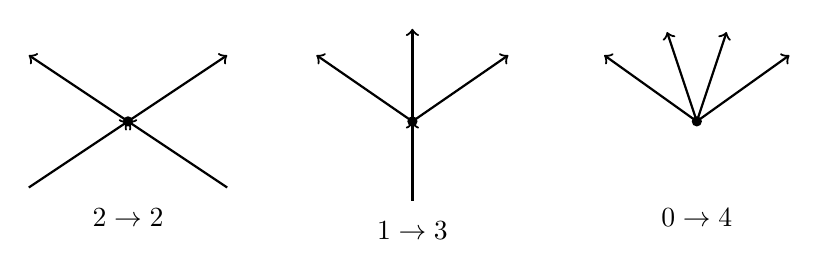
\begin{tikzpicture}[scale=0.84]
\fill (0,0) circle (2.2pt);
\draw[thick,->] (-1.5,-1.0) -- (0,0);
\draw[thick,->] (1.5,-1.0) -- (0,0);
\draw[thick,->] (0,0) -- (-1.5,1.0);
\draw[thick,->] (0,0) -- (1.5,1.0);
\node at (0,-1.45) {$2\to2$};
\begin{scope}[xshift=4.3cm]
\fill (0,0) circle (2.2pt);
\draw[thick,->] (0,-1.2) -- (0,0);
\draw[thick,->] (0,0) -- (-1.45,1.0);
\draw[thick,->] (0,0) -- (0,1.4);
\draw[thick,->] (0,0) -- (1.45,1.0);
\node at (0,-1.65) {$1\to3$};
\end{scope}
\begin{scope}[xshift=8.6cm]
\fill (0,0) circle (2.2pt);
\draw[thick,->] (0,0) -- (-1.4,1.0);
\draw[thick,->] (0,0) -- (-0.45,1.35);
\draw[thick,->] (0,0) -- (0.45,1.35);
\draw[thick,->] (0,0) -- (1.4,1.0);
\node at (0,-1.45) {$0\to4$};
\end{scope}
\end{tikzpicture}
\caption{Три локальные ориентации четырёхлучевой вершины взаимодействия.}
\end{figure}

Локальная интерпретация \(0\to4\) сама по себе не означает, что четыре частицы могут появиться из вакуума как физический процесс. Тем не менее необходимо просуммировать по всем возможным пространственно-временным положениям вершины. Когда предполагаемое внешнее состояние не может удовлетворять закону сохранения энергии, фазы от этих положений взаимно сокращаются.

\begin{classroomqa}
\lecturetimestamp{01:15:18}
\audiencequestion{Описывает ли ориентация с четырьмя исходящими линиями спонтанное появление четырёх частиц в конечном состоянии?}
\lecturerresponse{Это одна из локальных интерпретаций четырёхполевого оператора, но процесс без входящей энергии нарушает закон сохранения энергии. Когда складывают амплитуды от всех возможных пространственно-временных положений вершины, они взаимно сокращаются до нуля.}
\end{classroomqa}

\begin{classroomqa}
\lecturetimestamp{01:15:58}
\audiencequestion{Следуют ли законы сохранения энергии и импульса из самого вычисления?}
\lecturerresponse{Да. Интегрирование по вершине по всему времени обеспечивает сохранение энергии, а интегрирование по всему пространству — сохранение импульса. Сумма по положениям вершины обращается в нуль, если не выполняются оба закона сохранения.}
\end{classroomqa}

При соблюдении этих законов сохранения каждая диаграмма, допускаемая лагранжианом, вносит некоторый вклад в амплитуду. Величина этого вклада отчасти зависит от коэффициента каждого члена взаимодействия. Обозначим коэффициенты при кубическом и четвертичном членах через \(G_3\) и \(G_4\). Каждая трёхлучевая вершина даёт один множитель \(G_3\), а каждая четырёхлучевая вершина — один множитель \(G_4\). Поэтому диаграмма с \(V_3\) кубическими вершинами и \(V_4\) четвертичными вершинами имеет схематическую зависимость от констант связи
\begin{equation}
\mathcal{A}_{\mathrm{graph}}
\propto G_3^{V_3}G_4^{V_4}.
\end{equation}

Если эти константы связи малы, то диаграмма с малым числом вершин обычно даёт больший вклад, чем диаграмма с большим их числом. Каждая дополнительная вершина приносит ещё один малый множитель. Это даёт пертурбативной сумме шанс оказаться полезной: начинают с простейших диаграмм, а затем добавляют последовательно всё меньшие поправки.

Сходится ли полный ряд на самом деле, — трудный вопрос. Малые константы связи делают такое упорядочение правдоподобным, но сами по себе не решают всех проблем сходимости. При большой связи наивный ряд может вообще не работать. Такая неудача не показывает, что лежащая в основе теория неверна; она может показывать лишь то, что разложение по степеням константы связи было плохим способом её вычислять. Обсуждаемые методы наиболее непосредственно полезны, когда константы связи достаточно малы, так что диаграмма с четырьмя вершинами даёт вклад, гораздо меньший, чем диаграмма с двумя.

\begin{classroomqa}
\lecturetimestamp{01:19:24}
\audiencequestion{Можно ли рассматривать цветовую теорию таким же образом?}
\lecturerresponse{Да. Цветовая теория может быть сформулирована таким же образом и будет обсуждаться позже.}
\end{classroomqa}

\section{Пропагаторы, вершины и взаимодополняющие описания}

Следующая задача состоит в том, чтобы перечислить частицы и закодировать их динамику либо в лагранжиане, либо в правилах Фейнмана. Это две формы одной и той же информации. Квадратичные члены описывают распространение из одной точки в другую. Линия, представляющая такое распространение, называется пропагатором. Члены, содержащие три или более полей, описывают места, где линии встречаются. Эти точки встречи — вершины. Например,
\begin{equation}
\begin{aligned}
\text{quadratic term}
&\longleftrightarrow \text{propagator},\\
G_3\phi^3
&\longleftrightarrow \text{three-leg vertex}.
\end{aligned}
\end{equation}

Теорию можно задать, сопоставив каждой частице квантовое поле и записав один лагранжиан, содержащий все их массы и взаимодействия. Эквивалентно этому можно перечислить все пропагаторы, все разрешённые вершины и коэффициент, приписанный каждой вершине. Любой из этих списков говорит нам, какие процессы возможны и как приписывать амплитуды соответствующим графам.

Например, два электрона могут рассеяться, обмениваясь фотоном. Каждая электронная линия содержит вершину электрон--электрон--фотон, а фотонный пропагатор соединяет две вершины.\footnote{Диаграмма восстановлена по примеру из 01:21:38.}

\begin{figure}[htbp]
\centering
\begin{tikzpicture}[scale=0.95]
\draw[->] (-0.6,-0.2) -- (0.2,1.4);
\draw[->] (0.2,1.4) -- (-0.7,3.1);
\draw[->] (3.5,-0.2) -- (2.7,1.4);
\draw[->] (2.7,1.4) -- (3.6,3.1);
\fill (0.2,1.4) circle (2pt);
\fill (2.7,1.4) circle (2pt);
\draw[thick] (0.2,1.4) -- (2.7,1.4);
\node[above] at (1.45,1.4) {$\gamma$};
\node[left] at (-0.2,0.5) {$e^-$};
\node[right] at (3.1,0.5) {$e^-$};
\end{tikzpicture}
\caption{Рассеяние двух электронов посредством обмена фотоном.}
\end{figure}

Лагранжиан определяет амплитуду для этого графа и содержит симметрии и законы сохранения, которые её ограничивают. На рисунке с выделенным направлением времени частицы, помещённые внизу, образуют начальную конфигурацию, а частицы наверху — конечную конфигурацию.

\begin{classroomqa}
\lecturetimestamp{01:22:06}
\audiencequestion{В диаграмме Фейнмана частицы внизу образуют начальную конфигурацию, а частицы наверху — конечную?}
\lecturerresponse{Да. Внизу находится начальная конфигурация частиц, а наверху — конечная.}
\end{classroomqa}

Описание в терминах частиц и описание в терминах полей взаимодополняют друг друга, подобно тому как импульс и положение являются взаимодополняющими описаниями в обычной квантовой механике. Они описывают одну и ту же систему в разных базисах. Есть и соответствующая неопределённость: если число частиц задано точно, значение поля неопределённо; если значение поля задано точно, неопределённо число частиц. Ни одно описание не заменяет другое, и лагранжиан полезен в обоих.

\begin{classroomqa}
\lecturetimestamp{01:23:26}
\audiencequestion{Предсказываются ли константы связи теорией или определяются экспериментально?}
\lecturerresponse{Симметрии иногда могут связать одну константу связи с другой, но их численные значения, как правило, берутся из эксперимента.}
\end{classroomqa}

\section{Измеряемые исходные данные и обширные предсказания}

Сама по себе квантовая теория поля обладает изяществом и красотой. Но когда начинаешь перечислять факты---какие существуют частицы, каковы их массы и каковы их константы связи---, этот список оказывается беспорядочным. Это очень уродливый беспорядок, в котором почти нет согласованности, кроме той, что обеспечивается симметриями. Симметрии связывают разные типы частиц и их процессы, но лишь в ограниченной степени. Значительная часть этого перечня остаётся большим собранием сравнительно случайных фактов о несколько немотивированном наборе различных типов частиц.

\begin{classroomqa}
\lecturetimestamp{01:24:58}
\audiencequestion{Почему измеренным константам связи следует доверять так уверенно?}
\lecturerresponse{После того как константа связи измерена, изменение её значения приводит к неверным предсказаниям. Её величина проверяется многими расчётами, в которых она используется.}
\end{classroomqa}

Частиц слишком много, а это означает слишком много полей---слишком много с любой эстетической точки зрения. Их примерно сотня или около того. Имеется много констант связи, более или менее просто взятых из эксперимента, и много масс, значения которых разбросаны как попало. Между ними есть несколько соотношений, но лишь несколько.

Но как только вы их знаете, можно начинать вычислять. Как только они известны, этого достаточно: можно с большой точностью вычислять всё, что относится к этим частицам. Всё, что касается кварков, электронов, фотонов и остальных частиц, затрагивает атомную физику, физику частиц, ядерную физику, химию и, возможно, биологию. Объём исходных данных может быть больше, чем хотелось бы, но объём результата огромен.

\section{Квантовая электродинамика как пример теории возмущений}

Квантовая электродинамика даёт конкретный пример разложения по константе связи.

\begin{classroomqa}
\lecturetimestamp{01:26:12}
\audiencequestion{Сколько существует констант взаимодействия типа \(G_n\) для электронов и фотонов?}
\lecturerresponse{Существует одна элементарная константа взаимодействия: электрический заряд \(e\). Это коэффициент типа \(G_3\), приписанный вершине, в которой электрон входит, электрон выходит, а фотон испускается или поглощается.}
\end{classroomqa}

Опуская спинорные матрицы и индексы, взаимодействие схематически имеет следующий полевой состав
\begin{equation}
\mathcal{L}_{\mathrm{QED,int}}
\sim e\,(\text{electron bilinear})\,A,
\end{equation}
где \(A\) обозначает фотонное поле. Подробная структура с матрицами Дирака для аргумента подсчёта не нужна. Элементарное правило КЭД состоит в испускании или поглощении фотона электроном; все более сложные графы КЭД строятся повторным использованием этой единственной вершины.\footnote{Схематическая вершина восстановлена по 01:26:42; подробная матричная структура в источнике намеренно опущена.}

\begin{figure}[htbp]
\centering
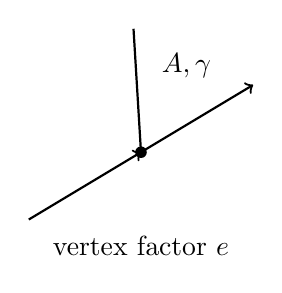
\begin{tikzpicture}[scale=0.95]
\draw[thick,->] (-1.5,-0.9) -- (0,0);
\draw[thick,->] (0,0) -- (1.5,0.9);
\draw[thick] (0,0) -- (-0.1,1.65);
\fill (0,0) circle (2.2pt);
\node[right] at (0.15,1.15) {$A,\gamma$};
\node at (0,-1.25) {vertex factor $e$};
\end{tikzpicture}
\caption{Элементарная вершина электрон--электрон--фотон в квантовой электродинамике.}
\end{figure}

\begin{classroomqa}
\lecturetimestamp{01:27:38}
\audiencequestion{А как обстоит дело с электрон--протонным рассеянием?}
\lecturerresponse{В элементарном атомном рассмотрении протон можно идеализировать как фиксированный, бесконечно тяжёлый точечный источник---тяжёлую частицу, намертво закреплённую на месте. Его собственная квантово-полевая динамика учитывается лишь тогда, когда включается внутренняя теория протонов и нейтронов.}
\end{classroomqa}

\begin{classroomqa}
\lecturetimestamp{01:28:30}
\audiencequestion{Может ли электрон двигаться почти со скоростью света относительно этого протона?}
\lecturerresponse{Да.}
\end{classroomqa}

Рассмотрим рассеяние фотона на электроне. В низшем порядке граф содержит две вершины электрон--электрон--фотон. Поэтому амплитуда пропорциональна \(e^2\):
\begin{equation}
\mathcal{A}_{\mathrm{lowest}}\propto e^2.
\end{equation}
Вероятность, или, что эквивалентно, зависимость сечения от константы связи, получается из квадрата модуля и пропорциональна \(e^4\):
\begin{equation}
P_{\mathrm{lowest}}\ \text{or}\ \sigma_{\mathrm{lowest}}
\propto e^4.
\end{equation}
При принятой безразмерной нормировке электрическая константа связи мала, поэтому реальное рассеяние значительно менее вероятно, чем простое прохождение фотона без рассеяния.

Уже на этом порядке есть два графа. В одном временном порядке входящий фотон поглощается, а исходящий испускается позже. В другом исходящий фотон испускается до того, как поглощается входящий. Обе амплитуды дают вклад.\footnote{Эти два временных порядка восстановлены по диаграммам из 01:28:42 и 01:30:18.}

\begin{figure}[htbp]
\centering
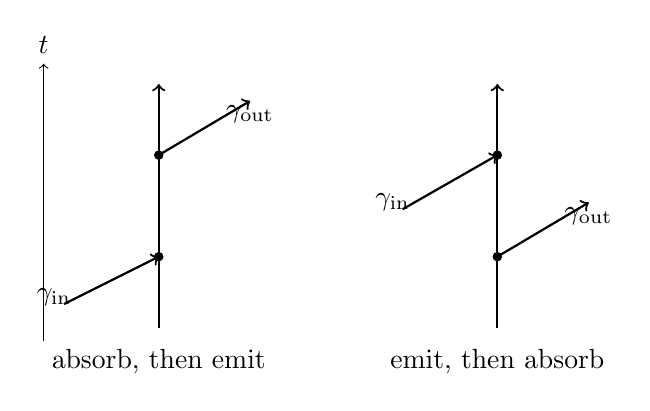
\begin{tikzpicture}[scale=0.86]
\draw[->] (-0.7,0) -- (-0.7,4.1) node[above] {$t$};
\draw[thick,->] (1.0,0.2) -- (1.0,3.8);
\fill (1.0,1.25) circle (2pt);
\fill (1.0,2.75) circle (2pt);
\draw[thick,->] (-0.4,0.55) -- (1.0,1.25);
\draw[thick,->] (1.0,2.75) -- (2.35,3.55);
\node[left] at (-0.15,0.65) {$\gamma_{\mathrm{in}}$};
\node[right] at (1.85,3.35) {$\gamma_{\mathrm{out}}$};
\node at (1.0,-0.3) {absorb, then emit};
\begin{scope}[xshift=5.0cm]
\draw[thick,->] (1.0,0.2) -- (1.0,3.8);
\fill (1.0,1.25) circle (2pt);
\fill (1.0,2.75) circle (2pt);
\draw[thick,->] (1.0,1.25) -- (2.35,2.05);
\draw[thick,->] (-0.4,1.95) -- (1.0,2.75);
\node[right] at (1.85,1.85) {$\gamma_{\mathrm{out}}$};
\node[left] at (-0.15,2.05) {$\gamma_{\mathrm{in}}$};
\node at (1.0,-0.3) {emit, then absorb};
\end{scope}
\end{tikzpicture}
\caption{Два временных упорядочения низшего порядка для электрон--фотонного рассеяния.}
\end{figure}

Следовательно, амплитуда низшего порядка представляет собой не один граф, а сумму двух:
\begin{equation}
\begin{aligned}
\mathcal{A}^{(2)}
&=
\mathcal{A}_{\mathrm{absorb\ then\ emit}}
+\mathcal{A}_{\mathrm{emit\ then\ absorb}},\\
\mathcal{A}^{(2)}&\propto e^2.
\end{aligned}
\end{equation}

Поправки более высокого порядка добавляют новые элементарные вершины. Дополнительный внутренний фотон, дважды присоединённый к электронной линии, добавляет два множителя \(e\), давая вклад, пропорциональный \(e^4\) в амплитуде и \(e^8\) в квадрате её модуля. Фотонная линия может также содержать электрон--позитронную вставку, что снова добавляет элементарные вершины и дополнительные степени \(e\). Это примеры, а не исчерпывающий список; дополнительный фотон можно присоединить во многих местах.\footnote{Структуры более высокого порядка восстановлены по 01:30:38--01:31:16.}

\begin{figure}[htbp]
\centering
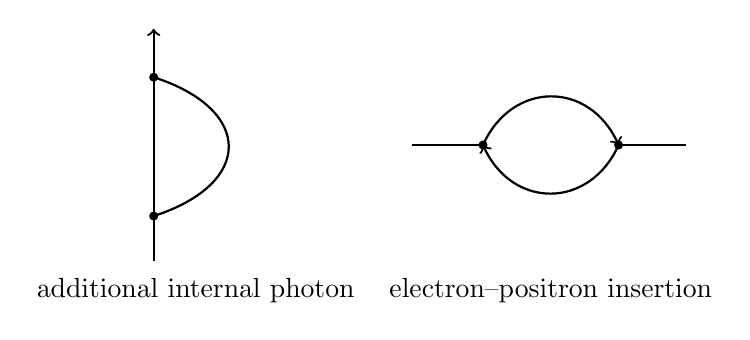
\begin{tikzpicture}[scale=0.82]
\draw[thick,->] (0.9,0.2) -- (0.9,3.8);
\fill (0.9,0.9) circle (2pt);
\fill (0.9,3.05) circle (2pt);
\draw[thick] (0.9,0.9) .. controls (2.45,1.4) and (2.45,2.55) .. (0.9,3.05);
\node at (1.55,-0.25) {additional internal photon};
\begin{scope}[xshift=5.1cm]
\draw[thick] (-0.2,2.0) -- (0.9,2.0);
\fill (0.9,2.0) circle (2pt);
\fill (3.0,2.0) circle (2pt);
\draw[thick,->] (0.9,2.0) .. controls (1.35,3.0) and (2.55,3.0) .. (3.0,2.0);
\draw[thick,->] (3.0,2.0) .. controls (2.55,1.0) and (1.35,1.0) .. (0.9,2.0);
\draw[thick] (3.0,2.0) -- (4.05,2.0);
\node at (1.95,-0.25) {electron--positron insertion};
\end{scope}
\end{tikzpicture}
\caption{Две структуры КЭД более высокого порядка, добавляющие элементарные вершины и дополнительные степени \(e\).}
\end{figure}

Таким образом, разложение КЭД идёт по последовательным степеням \(e^2\). Каждое аналогичное новое усложнение добавляет к амплитуде две степени электрического заряда. В используемой нормировке это делает такую поправку примерно в сто или в пару сотен раз меньшей по амплитуде, чем предыдущий порядок. Более сложные графы последовательно ослабевают, так что пертурбативная сумма имеет шанс оказаться полезной.

Вероятность не получают, возводя амплитуду каждого графа по отдельности в квадрат, а затем складывая эти квадраты. Сначала нужно сложить все амплитуды, вносящие вклад в один и тот же внешний процесс:
\begin{equation}
\mathcal{A}_{\mathrm{total}}=\sum_r\mathcal{A}_r.
\end{equation}
Лишь после этого берут
\begin{equation}
P=\left|\mathcal{A}_{\mathrm{total}}\right|^2
=\left|\sum_r\mathcal{A}_r\right|^2.
\end{equation}
Перекрёстные члены между различными графами — это интерференционные члены. Правило простое и существенное: сначала сложить, потом возвести в квадрат.

\section{К перечню частиц и Стандартной модели}

После того как введены пропагаторы, вершины, учёт степеней констант связи и интерференция, можно всерьёз приступить к описанию на языке физики элементарных частиц. Можно назвать частицы, задать их массы, записать лагранжианы, которым они подчиняются, опираясь отчасти на теорию, отчасти на эксперимент, и непосредственно в этих лагранжианах изучать их симметрии. Та же схема затем приводит к Стандартной модели и её свойствам.

\begin{classroomqa}
\lecturetimestamp{01:33:22}
\audiencequestion{Можно ли заменить постоянный массовый коэффициент \(m^2\) полем Хиггса?}
\lecturerresponse{Да. Это верная идея, и этот механизм будет обсуждаться позже.}
\end{classroomqa}

\begin{classroomqa}
\lecturetimestamp{01:33:42}
\audiencequestion{Могут ли соседние точки решётки \(x\) и \(x'\) относиться к двум разным моментам времени?}
\lecturerresponse{Да. Они могут быть соседями по времени; именно так на решётке представляется вертикальное распространение.}
\end{classroomqa}

Для соседних точек квадрат конечной разности содержит как одноузловые, так и межузловые члены:
\begin{equation}
\bigl[\phi(x)-\phi(x')\bigr]^2
=
\phi(x)^2+\phi(x')^2-2\phi(x)\phi(x').
\end{equation}

\begin{classroomqa}
\lecturetimestamp{01:33:56}
\audiencequestion{Какой член описывает частицу, просто стоящую на месте?}
\lecturerresponse{Одноузловые члены \(\phi(x)^2\) и \(\phi(x')^2\) в квадрате конечной разности соответствуют покою, тогда как межузловой член \(\phi(x)\phi(x')\) задаёт интерпретацию движения. Явный массовый член тоже вносит одноузловые факторы, соответствующие покою.}
\end{classroomqa}